\documentclass{article}

\usepackage{amsmath} % For math environments if needed
\usepackage{geometry} % For adjusting margins
\geometry{a4paper, margin=1in}
\usepackage{enumitem} % For better lists
\usepackage{pgfplots} % For plotting graphs with TikZ and PGFPlots
\pgfplotsset{compat=1.17}
\usepackage{tikz}
\usepackage{gensymb}
\usepackage{textcomp}
\usepackage[gen]{eurosym}

\title{Economics 101: Problem Set \#8 Solutions}
\author{Sean Balbale}
\date{\today}

\begin{document}
\maketitle

% =============================================================
\section*{Problem 1: AD and AS Analysis}
Discussion Question \#7 on p. 640 from the textbook:
\begin{quote}
  Use shifts of the AD and AS curves to explain
  \begin{enumerate}[label=(\alph*)]
    \item the U.S. experience of strong economic growth, full employment, and price stability in the late 1990s and early 2000s, and
    \item how a strong negative wealth effect from, say, a precipitous drop in house prices could cause a recession even though productivity is rising.
  \end{enumerate}
\end{quote}

\subsection*{Solution}

\begin{enumerate}[label=(\alph*)]
  \item \textbf{Growth with Price Stability.}
        During the late 1990s–early 2000s, rapid technological innovation and productivity improvements shifted the aggregate supply curve (\(AS\)) to the right. At the same time, booming business investment and household confidence shifted aggregate demand (\(AD\)) rightward as well. Because the rightward shifts of \(AS\) and \(AD\) were roughly equal, output rose substantially (toward and beyond full‐employment), but the price level remained stable.

  \item \textbf{Negative Wealth Effect Recession.}
        A large fall in house prices reduces household wealth and thus consumption. This shifts the \(AD\) curve to the left. In the short run, output falls below potential (creating a recessionary gap) and the price level declines. Productivity growth (rightward shift of \(AS\)) may moderate the price drop, but the leftward \(AD\) shift is sufficient to cause a recession even if \(AS\) is improving.
\end{enumerate}

\subsubsection*{Diagram 1(a): Growth with Price Stability}
\begin{center}
  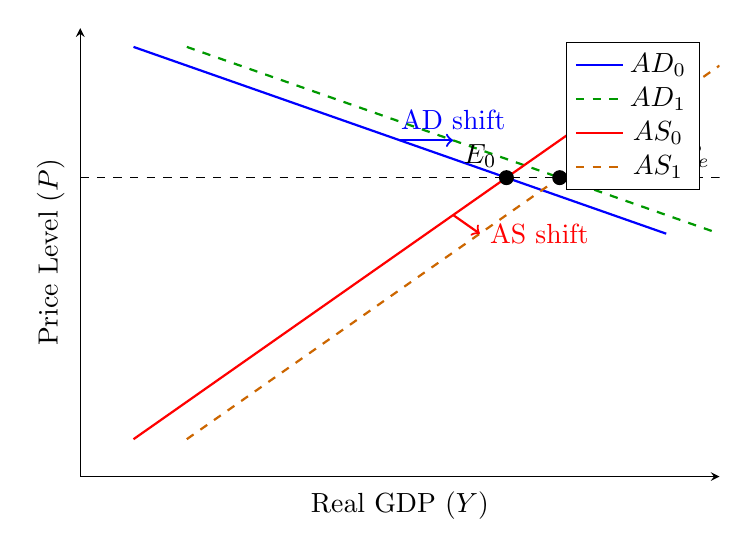
\begin{tikzpicture}
    \begin{axis}[
        width=0.8\textwidth,
        height=0.6\textwidth,
        xlabel={Real GDP (\(Y\))},
        ylabel={Price Level (\(P\))},
        xmin=0, xmax=12,
        ymin=0, ymax=12,
        axis lines=left,
        xtick=\empty,
        ytick=\empty,
        grid=both,
        grid style={gray!30},
        legend pos=north east
      ]
      % Original AD
      \addplot[domain=1:11, samples=100, blue, thick] {12 - 0.5*x};
      \addlegendentry{\(AD_0\)}
      % New AD
      \addplot[domain=2:12, samples=100, green!60!black, thick, dashed] {12.5 - 0.5*x};
      \addlegendentry{\(AD_1\)}
      % Original AS
      \addplot[domain=1:11, samples=100, red, thick] {x};
      \addlegendentry{\(AS_0\)}
      % New AS
      \addplot[domain=2:12, samples=100, orange!80!black, thick, dashed] {x - 1};
      \addlegendentry{\(AS_1\)}
      % Equilibrium points
      \addplot[only marks, mark=*, mark size=2.5, black] coordinates {(8,8)} node[above left] {\(E_0\)};
      \addplot[only marks, mark=*, mark size=2.5, black] coordinates {(9,8)} node[above right] {\(E_1\)};

      \draw[dashed,black] (axis cs:0,8) -- (axis cs:12,8)
      node[above left] {\(P_e\)};


      % Shift arrows
      \draw[->, thick, blue] (axis cs:6,9) -- (axis cs:7,9) node[above] {AD shift};
      \draw[->, thick, red] (axis cs:7,7) -- (axis cs:7.5,6.5) node[right] {AS shift};
    \end{axis}
  \end{tikzpicture}
\end{center}

\subsubsection*{Diagram 1(b): Negative Wealth Effect Recession}
\begin{center}
  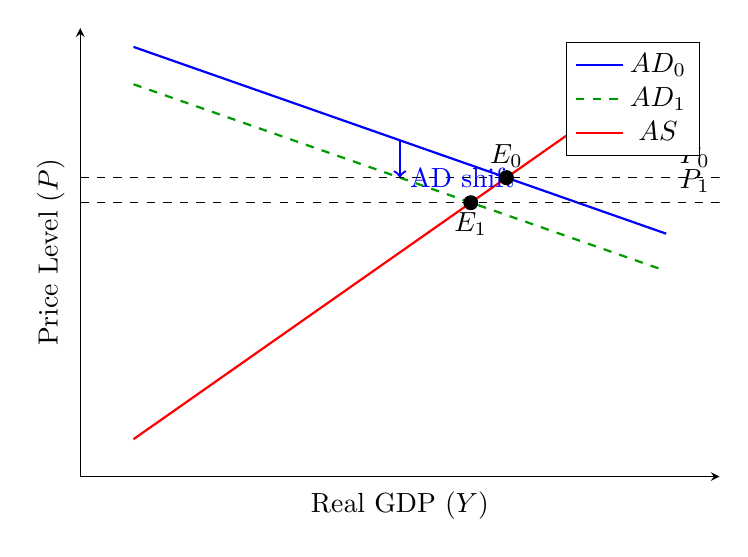
\begin{tikzpicture}
    \begin{axis}[
        width=0.8\textwidth,
        height=0.6\textwidth,
        xlabel={Real GDP (\(Y\))},
        ylabel={Price Level (\(P\))},
        xmin=0, xmax=12,
        ymin=0, ymax=12,
        axis lines=left,
        xtick=\empty,
        ytick=\empty,
        grid=both,
        grid style={gray!30},
        legend pos=north east
      ]
      % Original AD
      \addplot[domain=1:11, samples=100, blue, thick] {12 - 0.5*x};
      \addlegendentry{\(AD_0\)}
      % New AD (leftward shift)
      \addplot[domain=1:11, samples=100, green!60!black, thick, dashed] {11 - 0.5*x};
      \addlegendentry{\(AD_1\)}
      % AS curve unchanged
      \addplot[domain=1:11, samples=100, red, thick] {x};
      \addlegendentry{\(AS\)}
      % Equilibrium points
      \addplot[only marks, mark=*, mark size=2.5, black] coordinates {(8,8)} node[above] {\(E_0\)};
      \addplot[only marks, mark=*, mark size=2.5, black] coordinates {(7.33,7.33)} node[below] {\(E_1\)};

      \draw[dashed,black] (axis cs:0,8) -- (axis cs:12,8)
      node[above left] {\(P_0\)};

      \draw[dashed,black] (axis cs:0,7.33) -- (axis cs:12,7.33)
      node[above left] {\(P_1\)};

      % Shift arrow for AD
      \draw[->, thick, blue] (axis cs:6,9) -- (axis cs:6,8) node[right] {AD shift};
    \end{axis}
  \end{tikzpicture}
\end{center}

\section*{Problem 2: The Case Study of Spain}

In the attached article by Raphael Minder, Spain’s government abandons austerity and cuts taxes in 2014–16 to boost demand.  Answer the following:
\begin{enumerate}[label=(\Alph*)]
  \item Illustrate on an AD–AS diagram the Spanish economy’s 2014 output relative to full employment.
  \item The government wants to raise aggregate demand by $\euro$400 billion via lump‐sum tax cuts.  Given
        \[
          a = 150,\quad b = 0.80,\quad T = 50,\quad I = 300,\quad G = 100,\quad X = 40,\quad M = 50,
        \]
        by how much should taxes be cut?
  \item Show on your diagram the effects of this policy and explain.
  \item (Extra Credit) If AD increases by $\euro$400 billion, must equilibrium GDP also rise by $\euro$400 billion?  True or False, and calculate the exact new output level.
\end{enumerate}

\subsection*{Part A: Initial Equilibrium}

Compute the autonomous intercept:
\[
  A_0 = a - bT + I + G + (X-M)
  = 150 - 0.8\cdot50 + 300 + 100 + (40-50)
  = 500.
\]
Equilibrium output is
\[
  Y_0 = \frac{A_0}{1 - b}
  = \frac{500}{0.20}
  = 2500\text{ billion $\euro$}.
\]
If this is 74\% of full‐employment \(Y_{FE}\), then
\[
  Y_0 = 0.74\,Y_{FE}
  \;\Longrightarrow\;
  Y_{FE} = \frac{2500}{0.74}
  \approx 3378.38\text{ billion $\euro$}.
\]
Define the scaled variable \(Y' = Y/100\) (hundreds of billions):
\[
  Y'_0 = 25,
  \quad
  Y'_{FE} \approx 33.78.
\]

\begin{center}
  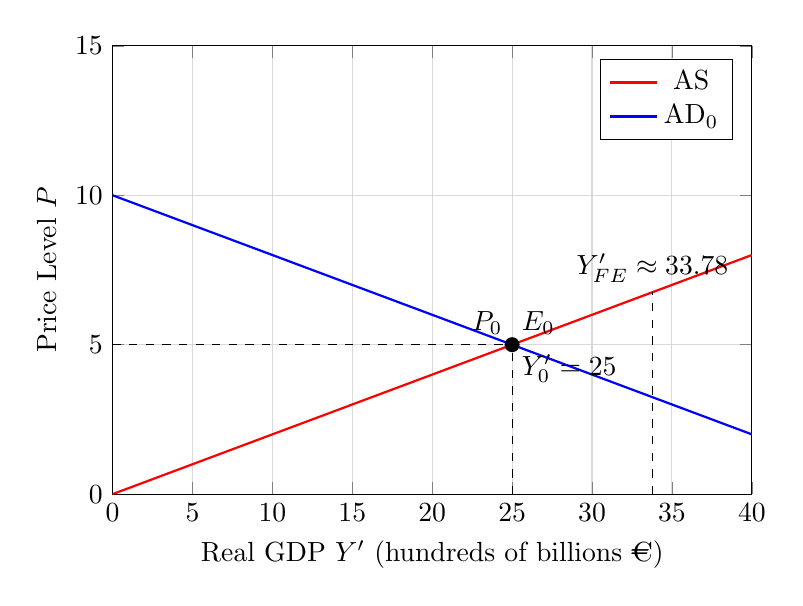
\begin{tikzpicture}
    \begin{axis}[
        width=0.8\textwidth,
        height=0.6\textwidth,
        xlabel={Real GDP \(Y'\) (hundreds of billions $\euro$)},
        ylabel={Price Level \(P\)},
        xmin=0, xmax=40,
        ymin=0, ymax=15,
        xtick={0,5,10,15,20,25,30,35,40},
        ytick={0,5,10,15,20},
        grid=both,
        grid style={gray!30},
        legend pos=north east
      ]
      % AS: P = (1/500) Y = 0.2 Y'
      \addplot[domain=0:40,samples=2,red,thick] {0.2*x};
      \addlegendentry{AS}

      % AD_0: P = 10 - (1/500)Y = 10 - 0.2 Y'
      \addplot[domain=0:40,samples=2,blue,thick] {10 - 0.2*x};
      \addlegendentry{AD$_0$}

      % Full‐employment vertical
      \draw[dashed,black] (axis cs:33.78,0) -- (axis cs:33.78,6.75)
      node[above] {\(Y'_{FE}\approx33.78\)};

      % Initial equilibrium
      \draw[dashed,black] (axis cs:25,0) -- (axis cs:25,5)
      node[below right] {\(Y'_0=25\)};
      \draw[dashed,black] (axis cs:0,5) -- (axis cs:25,5)
      node[above left] {\(P_0\)};

      \addplot[only marks,mark=*,mark size=2.5,black]
      coordinates {(25,5)} node[above right] {\(E_0\)};
    \end{axis}
  \end{tikzpicture}
\end{center}

\subsection*{Part B: Required Tax Cut}

The tax multiplier is
\[
  m_T = -\frac{b}{1-b}
  = -\frac{0.80}{0.20}
  = -4.
\]
To achieve \(\Delta Y = +400\),
\[
  \Delta Y = m_T\,\Delta T
  \;\Longrightarrow\;
  400 = -4\,\Delta T
  \;\Longrightarrow\;
  \Delta T = -100.
\]
A negative \(\Delta T\) means a \textbf{tax cut of $\euro$100 billion}.

\subsection*{Part C: Effects on the Diagram}

A $\euro$100 billion tax cut raises autonomous demand by
\[
  \Delta A = -\,b\,\Delta T = -0.8\times(-100) = 80,
\]
so \(A_1 = 580\) and
\[
  Y_1 = \frac{580}{0.20} = 2900\text{ billion $\euro$},
  \quad
  Y'_1 = 29
\]

\begin{center}
  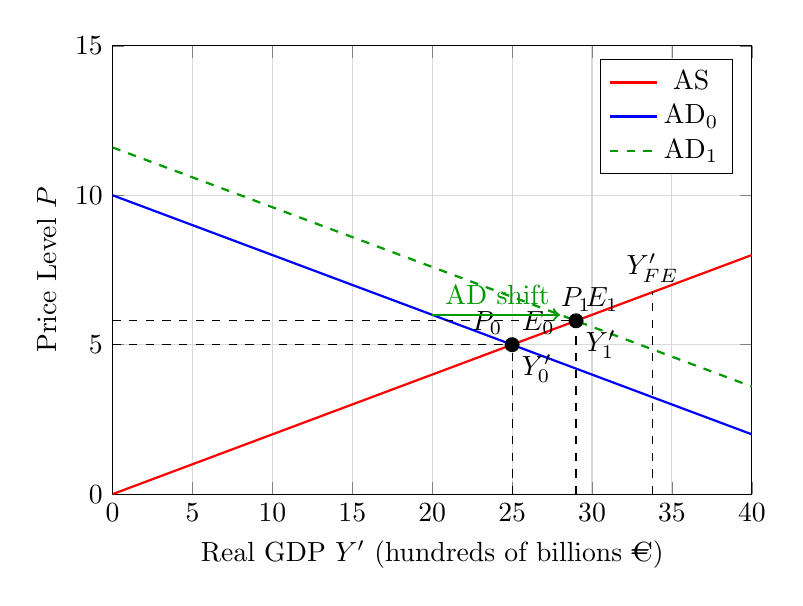
\begin{tikzpicture}
    \begin{axis}[
        width=0.8\textwidth,
        height=0.6\textwidth,
        xlabel={Real GDP \(Y'\) (hundreds of billions $\euro$)},
        ylabel={Price Level \(P\)},
        xmin=0, xmax=40,
        ymin=0, ymax=15,
        xtick={0,5,10,15,20,25,30,35,40},
        ytick={0,5,10,15,20},
        grid=both,
        grid style={gray!30},
        legend pos=north east
      ]
      % AS
      \addplot[domain=0:40,samples=2,red,thick] {0.2*x};
      \addlegendentry{AS}

      % AD0
      \addplot[domain=0:40,samples=2,blue,thick] {10 - 0.2*x};
      \addlegendentry{AD$_0$}

      % AD1
      \addplot[domain=0:40,samples=2,green!60!black,thick,dashed] {11.6 - 0.2*x};
      \addlegendentry{AD$_1$}

      % Full‐employment
      \draw[dashed,black] (axis cs:33.78,0) -- (axis cs:33.78,6.75)
      node[above] {\(Y'_{FE}\)};

      % Equilibria
      \draw[dashed,black] (axis cs:25,0) -- (axis cs:25,5)
      node[below right] {\(Y'_0\)};
      \addplot[only marks,mark=*,mark size=2.5,black]
      coordinates {(25,5)} node[above right] {\(E_0\)};
      \draw[dashed,black] (axis cs:29,0) -- (axis cs:29,5.8)
      node[below right] {\(Y'_1\)};
      \addplot[only marks,mark=*,mark size=2.5,black]
      coordinates {(29,5.8)} node[above right] {\(E_1\)};

      
      \draw[dashed,black] (axis cs:0,5) -- (axis cs:25,5)
      node[above left] {\(P_0\)};
      \draw[dashed,black] (axis cs:0,5.8) -- (axis cs:29,5.8)
      node[above] {\(P_1\)};

      % AD shift arrow
      \draw[->, thick, green!60!black] (axis cs:20,6) -- (axis cs:28,6)
      node[above left] {AD shift};
    \end{axis}
  \end{tikzpicture}
\end{center}

\subsection*{Part D: Extra Credit}

\textbf{False.}  The spending multiplier for any autonomous AD change is
\[
  k = \frac{1}{1-b} = 5,
\]
so a direct $\euro$400 billion increase in AD yields
\[
  \Delta Y = k \times 400 = 5 \times 400 = 2000\text{ billion $\euro$}.
\]
Starting from \(Y_0=2500\), the new equilibrium is
\[
  Y_1 = 2500 + 2000 = 4500\text{ billion $\euro$}
  \quad(\text{or }Y'_1 = 45\text{ on the graph}).
\]




\end{document}
